\section{Website}
In this section, we will not be providing any piece of code because of the verbose nature of web coding (Especially CSS). \\
All of the source code can be found in the Seafile folder dedicated to this project.

\subsection{Used Technologies}
\begin{itemize}
    \item HTML: to build the website skeleton
    \item Tailwind CSS: used instead of css to avoid \verb|CSS hell|
    \item Typescript: used instead of Javascript to write a safer code that won't fail on runtime
    \item Vue.js: used as frontend library to make reactivity easier
\end{itemize}


\subsection{Design}
We took inspiration from a \href{www.dribbble.com}{Dribbble.com} design of \href{https://dribbble.com/syahrulfalah}{Syahrul Falah}.

\begin{figure}[H]
    \centering
    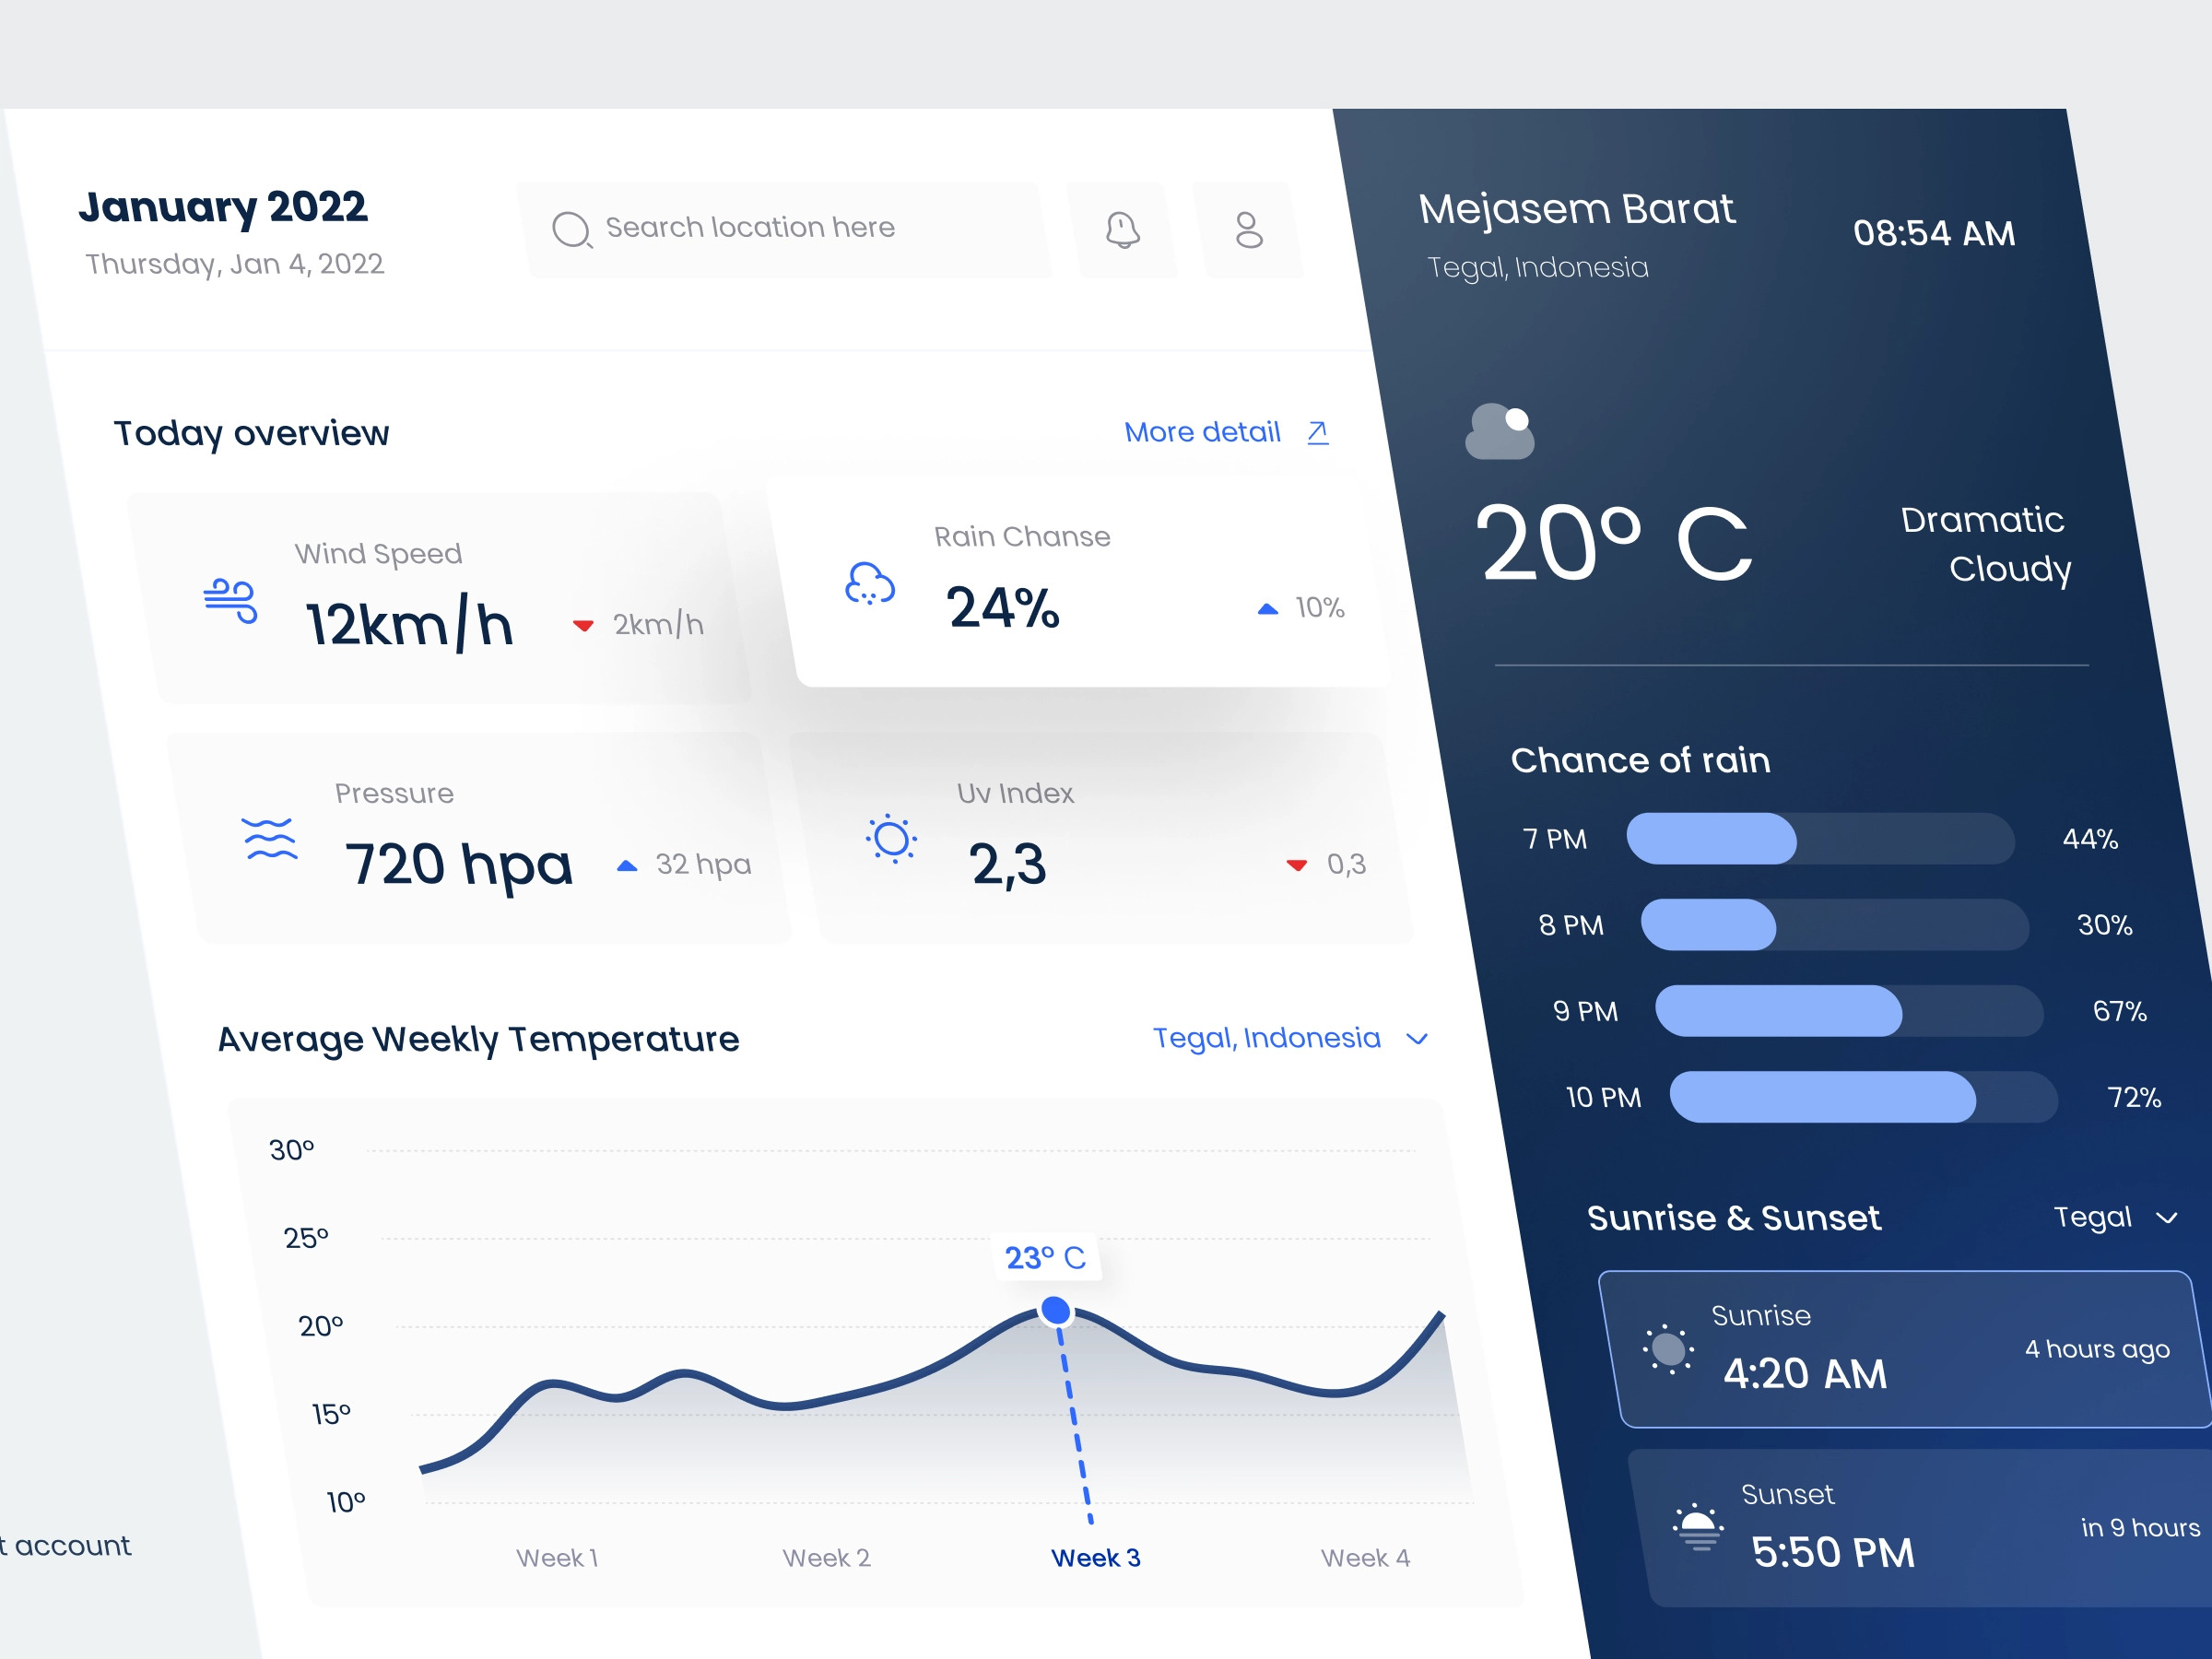
\includegraphics[width=.8\textwidth]{images/website/inspiration.jpg}
    \caption{Website reference design}
\end{figure}

\begin{figure}[H]
    \centering
    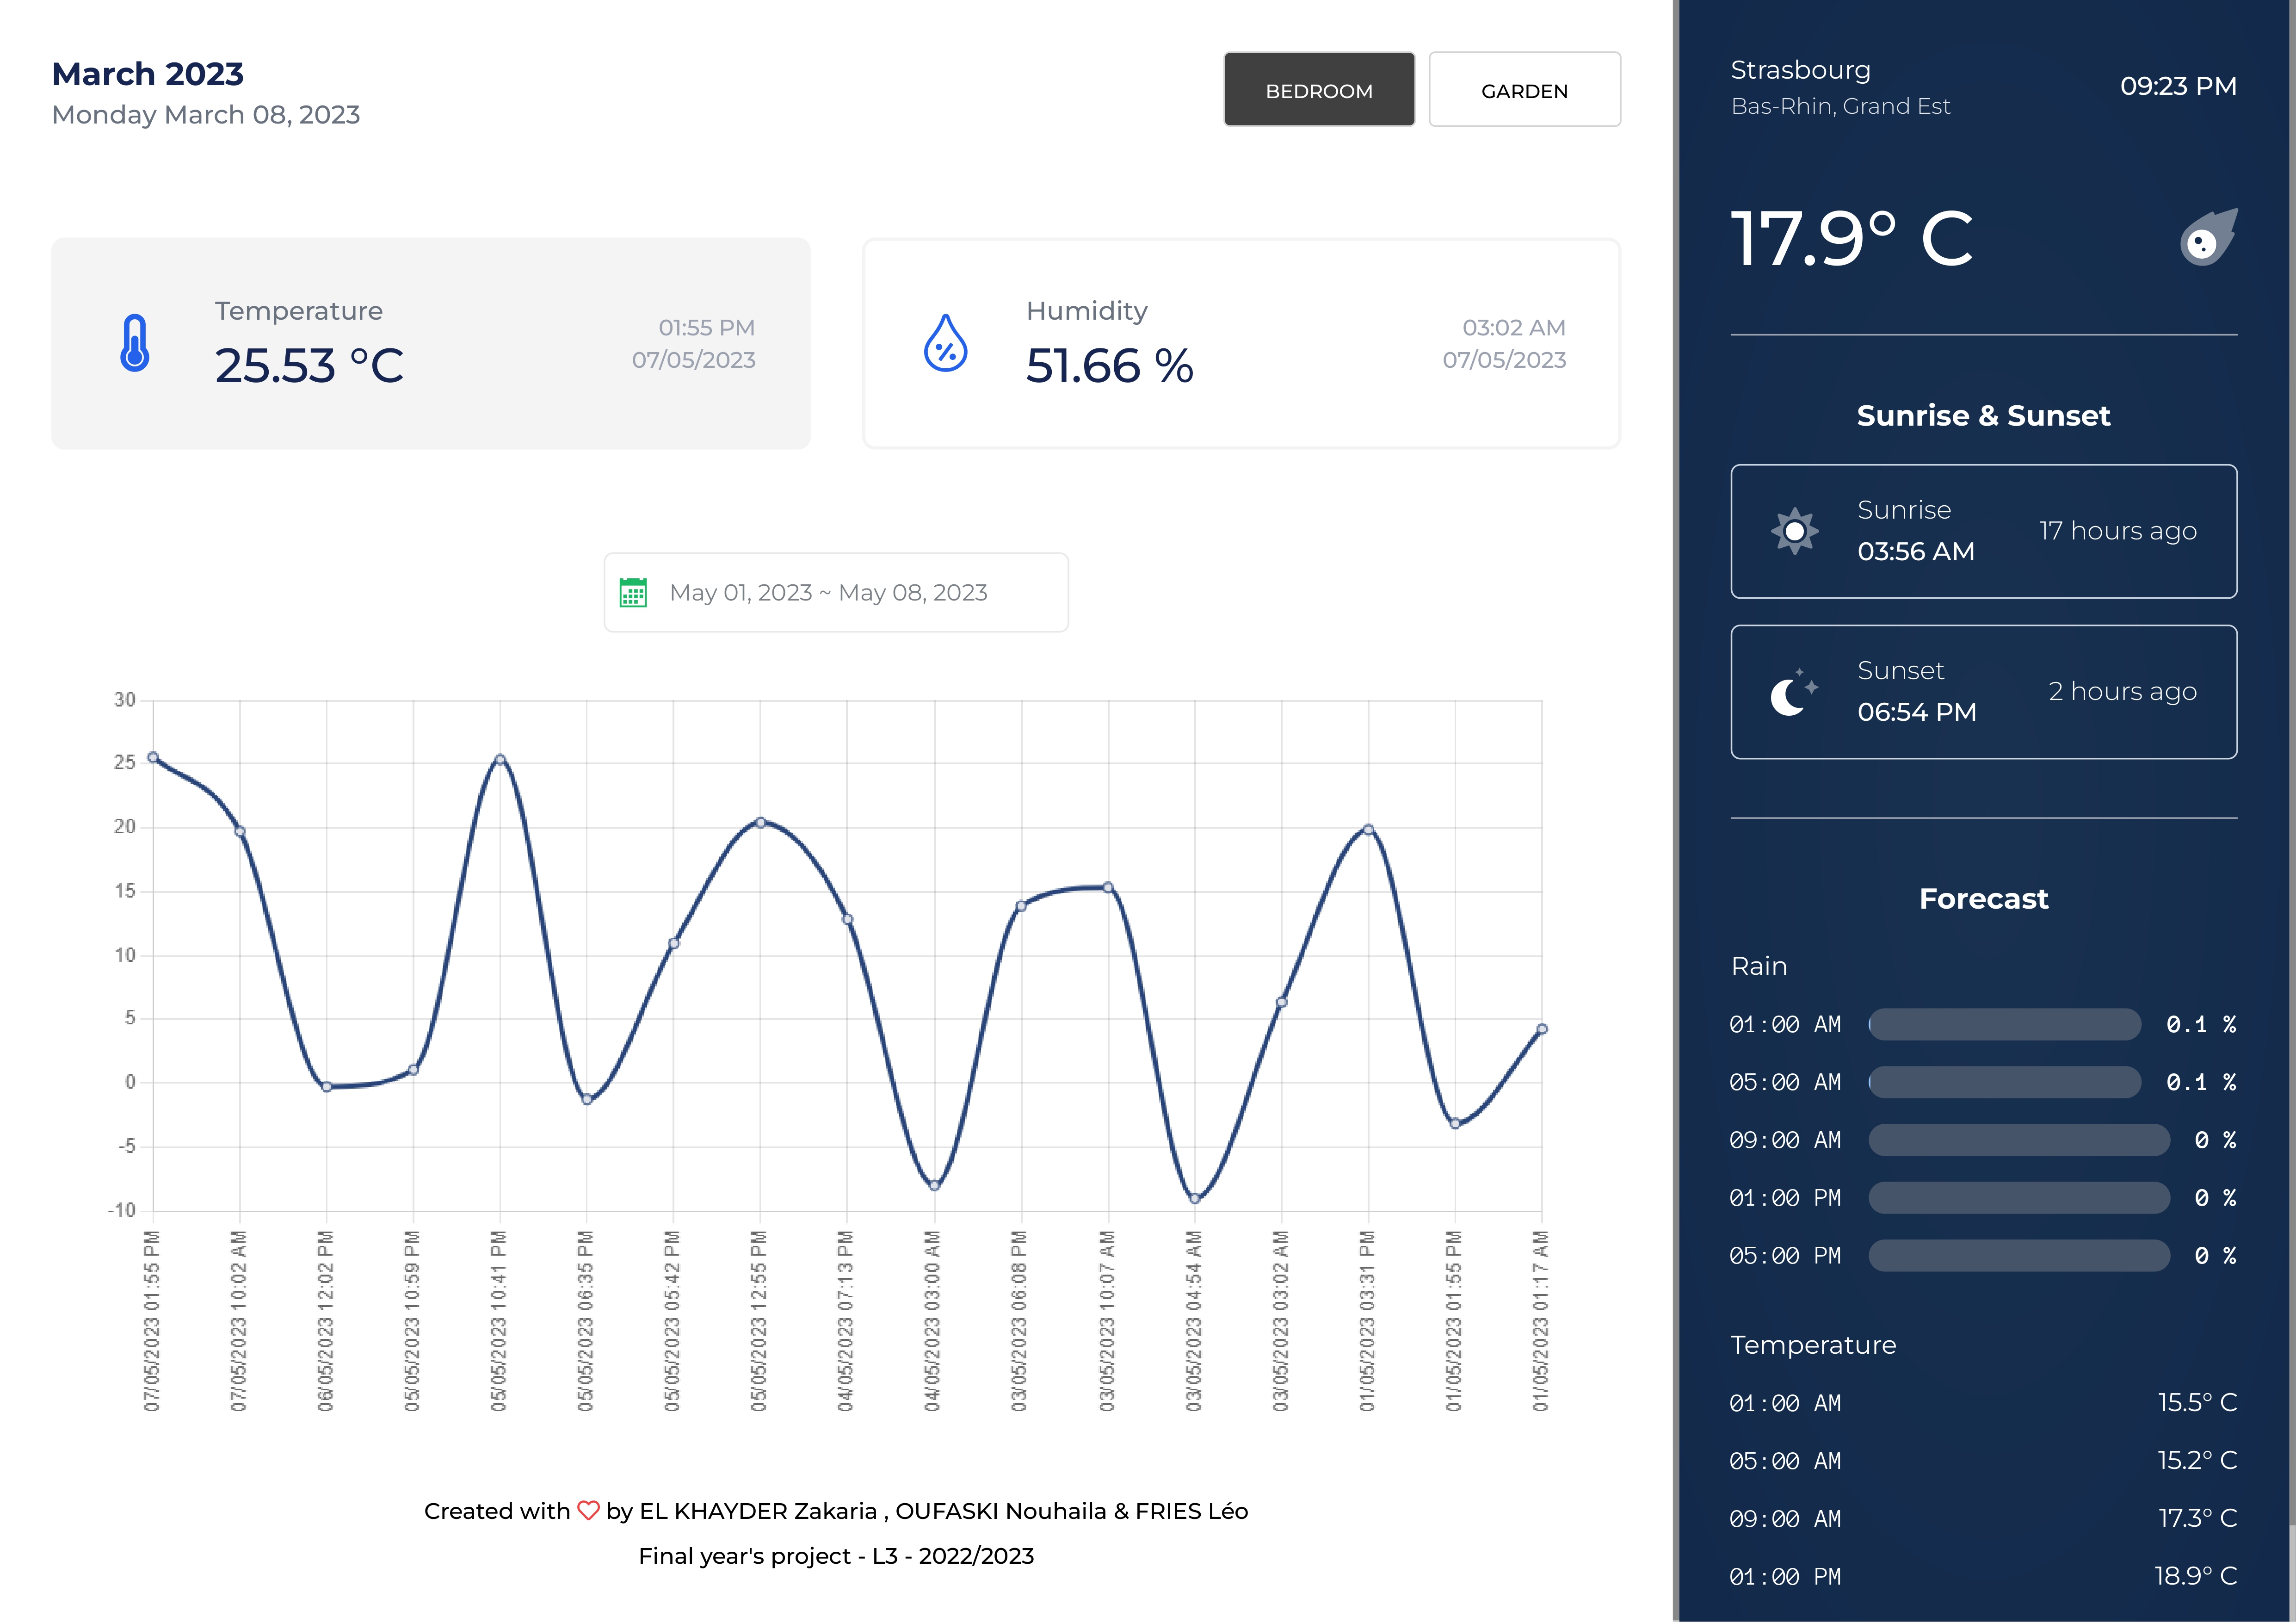
\includegraphics[width=\textwidth]{images/website/final_design.jpg}
    \caption{Website final result}
\end{figure}

\subsection{Functionalities}

\subsubsection{Geolocation}
We can get the user's current GPS location using the navigator's geolocation API, we can then reverse it back into an address using \href{https://geocode.maps.co}{geocode.maps.co} free API.

\subsubsection{Weather}
Using \href{https://open-meteo.com}{open-meteo.com} free API, we can get the current temperature for specific GPS coordinates.

\subsubsection{Sunrise \& sunset}
Using \href{https://sunrise-sunset.org}{sunrise-sunset.org} free API, we can get the sunrise \& sunset for specific GPS coordinates.

\subsubsection{Weather Forecast}
We can use \href{https://open-meteo.com}{open-meteo.com} free API to also get a weather forecast for specific GPS coordinates, such as rain probability and temperature forecast.

\subsubsection{Nodes data visualization}
We can parse the DB file that we can fetch from \verb|/api/db| and transform it into an object that we can use to analyze and visualize the data. \\
We used a graph to show different measurements of different nodes for a specific period that can be chosen with the date range selector. \\
We are also showing the latest measurement in hindsight for ease of use.